\section*{Problema 1}
\textbf{A lighthouse L is located on a small island 5 km north of a point A on a straight east-west shoreline. A cable is to be laid from L to point B on the shoreline 10 km east of A. The cable will be laid through the water in a straight line from L to a point C on the shoreline between A and B, and from there to B along the shoreline. (see Figure \ref{fig:problema1}). The part of the cable lying in the water costs \$5.000/km, and the part along the shoreline costs \$3, 000/km. Where should C be chosen to minimize the total cost of the cable?}

\begin{figure}[H]
    \centering
    \includegraphics[width=8cm]{Graphics/problem1.png}
    \caption{Problema 1}
    \label{fig:problema1}
\end{figure}

Llamnado x al segmento de recta $\overline{AC}$, y a $\overline{LC}$, entonces el segmento $\overline{CB}$ puede ser calculado como $10-x$. Las definiciones antes mencionadas se encuentran en la figura \ref{fig:problema1a}.

\begin{figure}[H]
    \centering
    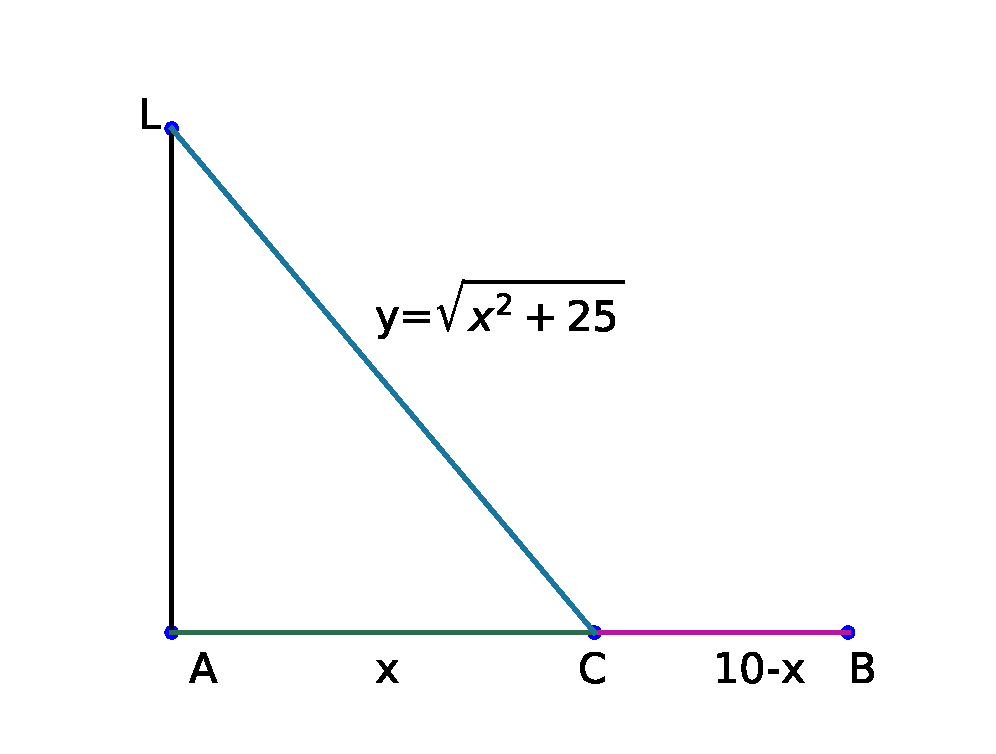
\includegraphics[width=10cm]{Graphics/problem1_graph.eps}
    \caption{Representación de las definiciones de cada segmento de linea.}
    \label{fig:problema1a}
\end{figure}

Definiendo la función de costo de cada linea se obtiene la función \ref{eq:problema1_definicion}.

\begin{equation}
    C(x) = 3000(10-x) + 5000 \sqrt{x^2+25} \label{eq:problema1_definicion}
\end{equation}

Realizando la derivada con respecto a x de le función \ref{eq:problema1_definicion} para encontrar los valores críticos.

\begin{align*}
    \frac{dC(x)}{dx} & = -3000 + \frac{5000(x)}{\sqrt{x^2+25}}
\end{align*}

Encontrando los valores criticos se obtiene lo siguiente:
\begin{align*}
    -3000 + \frac{5000(x)}{\sqrt{x^2+25}} & =0               \\
    \frac{5000(x)}{\sqrt{x^2+25}}         & = 3000           \\
    5x                                    & = 3\sqrt{x^2+25} \\
    25x^2                                 & = 9(x^2+25)      \\
    16x^2     -225                        & = 0              \\
    (4x-15)(4x+15)                        & = 0              \\
    x_1                                   & = \frac{15}{4}   \\
    x_2                                   & = -\frac{15}{4}
\end{align*}

La solución $x_2$ es despreciada, ya que su sentido físico no admisible, por lo tanto el punto C debe estar a 3.75km del punto A.
